\section{Exploring the incidents' geographical distribution}

\subsection*{Question 1.1}
\textit{Are there high variations of incidents densities over Seattle? Which are the low-density zones? Which are the high density zones?}

The visualization uses a map of the city of Seattle (a scatterplot that uses the maps from OpenStreetMap for the background):
each point in the dataset is visualized as a circle on the map.
Columns and rows are used to encode respectively longitude and latitude.
The size of the circles is set to the minimum, the opacity to the value $8\%$.
Size and opacity does not encode any particular information, but the combination of small size, opacity and zoom level allows to visualize an approximation of the density of incidents.
The zoom level is small in order to get an overview of the entire city that fits the screen, size and opacity are regulated accordingly.

\begin{figure}[h]
	\centering
	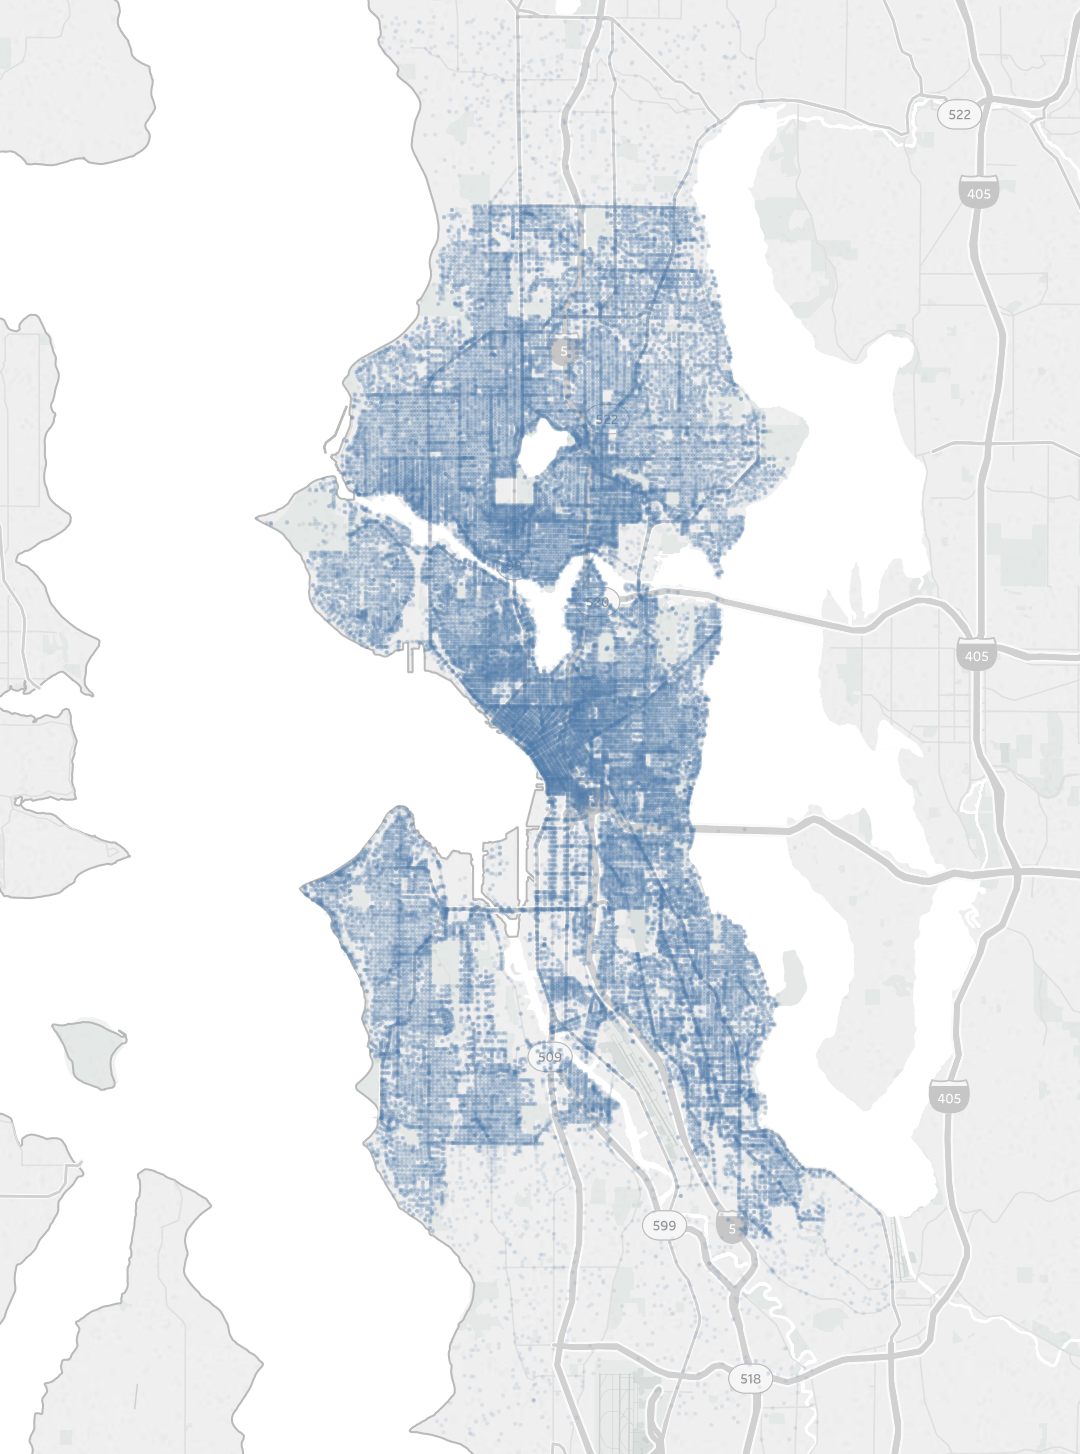
\includegraphics[width=.75\columnwidth]{figures/1_1_geographical_distribution_incidents}
	\caption{Geographical distribution of the incidents in Seattle. The screenshot is taken from the sheet called \textit{Geographical Distribution of Incidents in Seattle} in Tableau.}
	\label{fig:1_1_geographical_distribution_incidents}
\end{figure}

\cref{fig:1_1_geographical_distribution_incidents} shows that there are indeed variations in the density of incidents in Seattle:
\begin{itemize}
    \item The regions in the very north and south of the city have a very small number of incidents. These areas are already outside the borders of Seattle. We suspect they are not usually covered by the police of Seattle, so the dataset may not contain all the incidents that occurred in the those areas.
    \item Incidents seems to be more concentrated in the central area of the city, around the Elliott Bay, and immediately to its north.
    \item Outside the city center, the main roads have a higher number of incidents than the surrounding areas (in particular in the south part of the city).
    \item The density of incidents in the rest of the city is lower and seems to be approximately uniform.
\end{itemize}

The visualization answers the question, but it is not optimal.
A better solution would be to use a density plot which is able to visualize better the differences of incidents' densities in the city.
Unfortunately, Tableau does offer density plots, so I tried to approximate it.

\subsection*{Question 1.2}
\textit{Are there high variations of incidents densities over Seattle for specific types of incidents? Which are these types and which are the variations you found?}
